\chapter{Introduction}
\label{ch:intro-ref}

This chapter introduces the problem MandiSense AI addresses, states the objectives against which the project is judged, defines the problem precisely, and gives a roadmap of the thesis.

\section{Background}
\label{sec:background}

India's fresh-produce markets are run through regulated wholesale yards, the Agricultural Produce Market Committee (APMC) mandis. A farmer in Kolar district who harvests tomato has, on any morning, a handful of yards within a day's reach, a truck that costs money per kilometre, a crop that loses weight and value every day it waits, and a price that changes daily by amounts large enough to matter more than the transport. The state publishes mandi prices through the national Agmarknet portal~\cite{agmarknet}, and prices in these crops are among the most volatile in the economy~\cite{birthal2019}. Figure~\ref{fig:kolar} shows five years of tomato at Kolar APMC: the modal price ranged from Rs~\KolarMin{} to Rs~\KolarMax{} per quintal, and on \KolarMissing{} of \KolarDays{} calendar days the mandi posted no price at all.

\begin{figure}[!b]
    \centering
    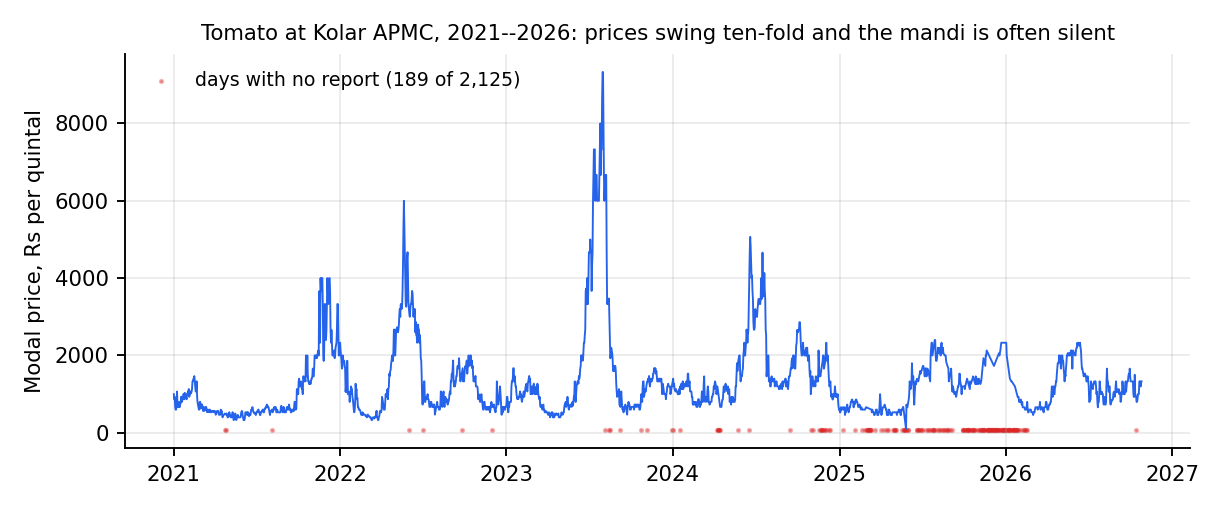
\includegraphics[width=0.95\textwidth]{figures/fig_intro_kolar_tomato.png}
    \caption{Modal price of tomato at Kolar APMC (Agmarknet, 2021--2026). The red marks along the bottom are days with no report; a farmer cannot tell from the portal whether such a day means no trade or no data.}
    \label{fig:kolar}
\end{figure}

Information matters to sellers. Field studies from southern India and West Africa found that when traders and fishermen could compare prices across markets by mobile phone, price dispersion fell and welfare rose~\cite{jensen2007,aker2010}. A price portal that lists yesterday's quotes is a weak form of that information. It gives a number for each market but not the answer to the farmer's question, which is \emph{where should this load go, and should it go today}.

Machine learning has been applied extensively to agricultural price forecasting, with hybrid models that decompose a price series and forecast the pieces reporting very large gains~\cite{ray2023,sathe2025,celik2025,wu2026}. This project took a different starting point. A forecast is useful only through the decision it supports, so the quantity to be judged is the money a farmer ends up with, and that has to be measured on data the model could not have seen.

Three further needs follow from how farmers and traders actually use such a tool. First, a number is not advice: a farmer who reads Kannada, or a trader short of time, wants a plain recommendation with reasons, and language models can write one, but they also invent figures, so any brief they write must be checked against the evidence before it is shown. Second, crops do not move alone. A shortage of tomato can pull on the price of onion or potato, and a trader holding several crops needs to know whether such links are real or are the common market movement seen through a different lens. Third, advice has to be inspectable and has to reach the farmer where they are: a farmer asks why a faraway mandi beats the nearest one, an examiner asks what happens if everyone follows the advice, and a recommendation that waits on a web page nobody opens helps no one. Chapters~\ref{ch:method}--\ref{ch:results} treat all three needs with the same discipline as the main engine: claims are tested on held-out data and withheld when the evidence does not support them.

\section{Objectives}
\label{sec:objectives}

\noindent \textbf{Primary objective.} To build and evaluate a decision-support system that recommends, for a farmer's crop and location, the mandi and the holding period that maximise net revenue, and that states a revenue floor the recommendation is verified to respect.

\noindent \textbf{Specific objectives.}
\begin{enumerate}
    \item To construct, by 31 October 2026, a clean panel from the real Agmarknet history for the Bengaluru--Kolar belt (at least 30,000 mandi-days, four crops) with every cleaning step and exclusion recorded.
    \item To formulate net revenue per quintal from price, shrinkage, transport cost and the probability that a market is silent, and to train a market-choice model on it, measuring regret against a hindsight oracle on at least 500 held-out days per crop.
    \item To test, with block-bootstrap intervals and Holm-corrected paired tests, whether (a) realised-revenue labels and (b) a decision-focused loss improve on conventional training, and to report the result whether or not it is favourable.
    \item To derive revenue floors whose empirical violation rate is within two percentage points of the nominal level at 10\% over a walk-forward evaluation.
    \item To deliver the engine through a FastAPI service and a trilingual (English, Kannada, Hindi) web application for farmers and traders, with automated tests and a reproducible pipeline from raw data to served model.
    \item To audit published decompose-then-forecast price models for look-ahead leakage and to benchmark against a zero-shot foundation model.
    \item To build an LLM-based \emph{decision intelligence} service that turns the engine's evidence into a structured brief (action BUY, SELL, HOLD or WAIT, a confidence level, and factors that each cite their evidence), and to verify every figure in a brief against the evidence it was given, with a deterministic fallback when the model fails or its answer is not grounded. Success is measured by the share of explanation sentences kept after an independent faithfulness judge in English, Kannada and Hindi, and by the judge catching at least eight of nine deliberately corrupted explanations without rejecting faithful ones.
    \item To estimate \emph{cross-commodity spillover}, that is, how a supply shock in one of five crops transmits to the prices of the others after removing the common market factor and seasonality, for all 40 ordered source--target--direction combinations, with episode-level bootstrap intervals and false-discovery-rate control, publishing an edge only when at least eight shock episodes support it.
    \item To make the advice inspectable and auditable with five features built on the engine: a per-quintal breakdown whose parts add up to the served net revenue (within Rs~1); a what-if simulator that re-prices the advice under the farmer's own costs and reports the cost at which it changes; a day-by-day track record on days the advice was not fitted on, whose headline numbers reproduce the back-test; a silence tax per mandi; and a crowd simulator for many farmers following the same advice, with every scenario parameter stated.
    \item To deliver a dated morning digest in English, Kannada and Hindi through a free messaging channel (Telegram) built only from ingested data, giving selling advice only for crops whose evidence is strong, and to demonstrate it end to end with a delivery log. A field pilot with farmers is outside this objective.
\end{enumerate}

\section{Problem Statement}
\label{sec:problem-statement}

A seller of a perishable crop faces a joint choice of destination $m\in\mathcal{M}$ and holding days $k\in\{0,1,2,3\}$, or sale at the farm gate. Define the net revenue per quintal of action $(m,k)$ on day $t$ as the price realised at $m$ on day $t+k$, less the value lost to shrinkage, less transport cost, with a penalty when $m$ does not report. The farmer observes only past prices, and observes them only for markets and days that were reported. The problem is to choose an action that maximises realised revenue and to state, before the sale, a floor below which revenue will fall only rarely.

Three properties make the problem harder than forecasting a price series. First, \emph{selective reporting}: the price at a market is missing on the days it is least informative to the model, and a model trained only on posted prices learns that every market is always open. Second, \emph{the object of interest is a decision}, so the error that matters is regret, the revenue lost relative to the best action in hindsight, not the squared error of a price. Third, \emph{a recommendation without an error statement is not usable}: a farmer who gambles a harvest needs to know how bad the outcome can be.

\noindent \textbf{Scope.} Four crops (tomato, onion, potato, ginger) in the Bengaluru--Kolar belt; daily modal prices; the Agmarknet source only; offline evaluation on history. Two supporting services are in scope: a grounded decision brief written by a language model over the engine's evidence, and an estimate of how supply shocks in one crop spill over to the others. Five insight features that explain and audit the advice, and a Telegram morning digest, are also in scope. Garlic was excluded from market choice because only one mandi had enough reported days, so no choice between markets exists. Field trials with farmers, price effects of the system's own advice, and live market access are outside the scope.

\section{Summary}
\label{sec:intro-summary}

The chapter argued that the farmer's question is a decision under uncertainty with missing data and that judging it by forecast error misses the point. The primary objective is a recommendation with a verified floor, supported by ten measurable objectives, the last four being a grounded language-model decision brief, a cross-commodity spillover estimate, five features that explain and audit the advice, and a morning digest on a free messaging channel. Chapter~\ref{ch:lit} reviews related work and the gaps this project fills. Chapter~\ref{ch:method} sets out requirements, the proposed method, architecture, dataset and evaluation design. Chapter~\ref{ch:plan} documents planning and management. Chapter~\ref{ch:impl} describes implementation, integration and testing. Chapter~\ref{ch:results} reports results, including those that did not work. Chapter~\ref{ch:concl} concludes with learnings, limitations, future work and the mapping to engineering outcomes and sustainable development goals. The appendices hold code, the survey instrument, evaluation tables, dataset description, outcome mapping and the similarity record.
